\documentclass[12pt]{article}
\usepackage[italian]{babel}
\usepackage[dvipsnames]{xcolor}
\usepackage[utf8]{inputenc}
\usepackage{hyperref}
\usepackage{graphicx}
\usepackage{float}
\usepackage{incgraph}
\usepackage{listings} % syntax highlighting
\usepackage{tabularx}
\usepackage{minted}
% https://tex.stackexchange.com/a/343329/232428
\renewcommand\tabularxcolumn[1]{m{#1}}% for vertical centering text in X column


\definecolor{dkgreen}{rgb}{0,0.6,0}
\definecolor{gray}{rgb}{0.5,0.5,0.5}
\definecolor{mauve}{rgb}{0.58,0,0.82}
\definecolor{LightGray}{rgb}{0.97,0.97,0.97}

% from https://gist.github.com/vsimko/fcc84e1e4f8e750746caa34b802db5a7
\lstdefinelanguage{SPARQL}{
  basicstyle=\small\ttfamily,
  backgroundcolor=\color{LightGray},
  columns=fullflexible,
  breaklines=false,
  sensitive=true,
  numbers=left,
  % --------------------------
  frame=bt,
  aboveskip=1em,
  belowskip=1em,
  xleftmargin=.5em,
  xrightmargin=.5em,
  framexleftmargin=.5em,
  framextopmargin=.5em,
  framexbottommargin=.5em,
  framexrightmargin=.5em,
  % --------------------------
  tabsize = 2,
  showstringspaces=false,
  morecomment=[l][\color{gray}]{\#},       % comments
  morecomment=[n][\color{blue}]{<http}{>}, % uris
  morestring=[b][\color{OliveGreen}]{\"},  % strings
  % -------------------------- variables
  keywordsprefix=?,
  classoffset=0,
  keywordstyle=\color{Sepia},
  morekeywords={},
  % -------------------------- prefixes
  classoffset=1,
  keywordstyle=\color{Purple},
  morekeywords={rdf,rdfs,owl,xsd,purl,foaf},
  % -------------------------- keywords
  classoffset=2,
  keywordstyle=\color{MidnightBlue},
  morekeywords={
    SELECT,CONSTRUCT,DESCRIBE,ASK,WHERE,FROM,NAMED,PREFIX,BASE,OPTIONAL,
    FILTER,GRAPH,LIMIT,OFFSET,SERVICE,UNION,EXISTS,NOT,BINDINGS,MINUS,a,
    DISTINCT
  }
}


\newcommand\blankpage{
    \null
    \thispagestyle{empty}
    \newpage
    }

\author{Davide Mauri}
\date{January 2023}

\begin{document}

\begin{titlepage}

\thispagestyle{empty}

\centerline {\Large{\MakeUppercase{ Università DEGLI STUDI DI TORINO}}}
\vskip 20 pt

\centerline {\Large{\textsc DIPARTIMENTO DI INFORMATICA}}

\vskip 20 pt

\centerline {{\textsc SCUOLA DI SCIENZE DELLA NATURA}}

\vskip 20 pt

\centerline {\Large{\textsc Corso di Laurea Magistrale in Informatica}}

\vskip 50 pt


%\begin{tabular}{ccc}
\centerline {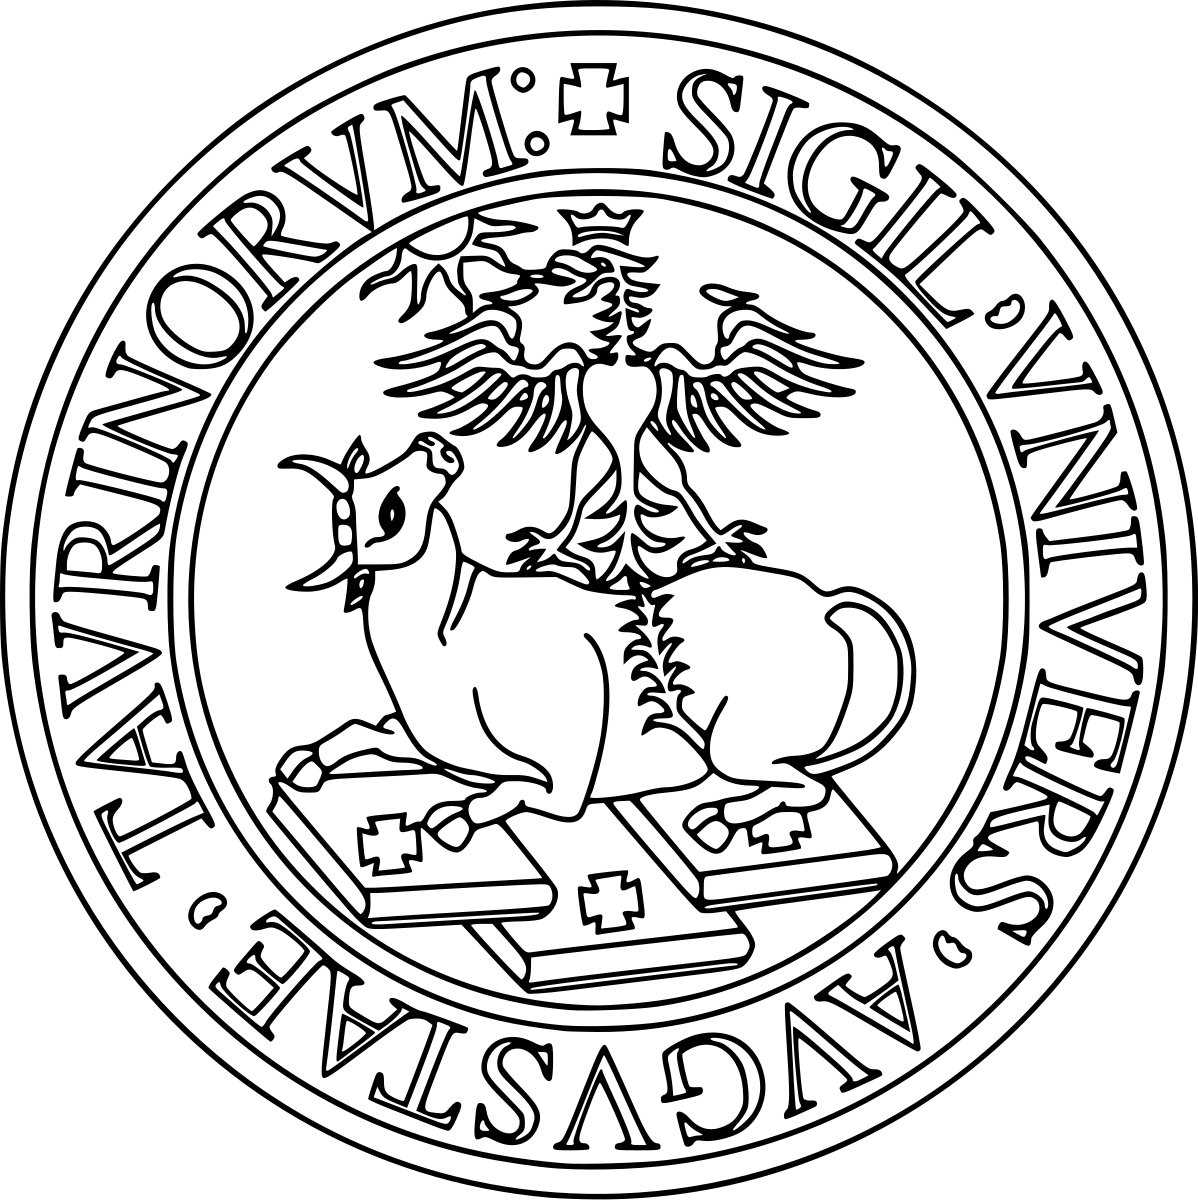
\includegraphics[width=4cm]{files/Unito-logo.png}}
%   \end{tabular}

\vskip 2cm

\centerline {\Large {\bf Progetto Modellazione Concettuale del Web Semantico}}

\vskip 1.7cm

\centering{Davide \textsc{Mauri}}

\vskip 2.7cm


\centerline{ANNO ACCADEMICO}
\vskip 0.1cm
\centerline{2022/2023}

\end{titlepage}

\tableofcontents

\newpage
\section{Introduzione}
Questo documento è la documentazione richiesta per lo sviluppo del progetto del corso Modellazione Concettuale del Web Semantico tenuto dall'Università degli Studi di Torino nell'anno accademico 2022/2023. L'unico autore di quanto presentato è Davide Mauri.

\'E disponibile un repository github all'indirizzo \url{https://github.com/Davidesfed/CollectibleCardGameOntology} che contiene tutto ciò che viene presentato in questo documento, documentazione LODE compresa.

\newpage
\section{Motivazioni}
Il dominio scelto riguarda i giochi di carte collezionabili (in inglese CCG “Collectible Card Game” oppure TCG “Trading Card Game”). Questi sono giochi di carte dove, al contrario dei classici come "Poker" o "Scala Quaranta", ogni giocatore utilizza un mazzo costruito da sé stesso, scegliendo le carte da un bacino generalmente molto più grande della dimensione effettiva di un mazzo. Questa personalizzazione obbligatoria sembra\footnote{Tesi di laurea "Il collezionismo come processo di consumo: il caso delle carte da gioco Pokémon": \url{http://hdl.handle.net/20.500.12608/41167}} essere una delle caratteristiche più apprezzate dai giocatori, che li porta quindi a voler spendere soldi per acquistare nuove carte in modo da migliorare gradualmente i propri mazzi.

Io stesso, fin da piccolo, ho sempre apprezzato proprio queste meccaniche e crescendo ho capito che mi hanno aiutato a sviluppare alcune capacità che sono riutilizzabili nella vita di tutti i giorni\footnote{Articolo "Collectible Card Games as Learning Tools": \url{https://doi.org/10.1016/j.sbspro.2012.06.130}}.
Inoltre alcuni studi asseriscono che i CCG abbiano anche potenzialità in ambito scolastico, per facilitare la comprensione di particolari argomenti\footnote{Articolo "A trading-card game teaching about host defence": \url{https://doi.org/10.1046/j.1365-2923.2002.01384.x}} oppure come sistema di motivazione degli studenti tramite ricompense\footnote{Articolo "Trading Card Game": \url{http://maiga.athabascau.ca/publication/Conference-2016-ICCE2016.pdf}}. Da questi fatti si evince che i giochi di carte collezionabili abbiano un valore intrinseco certamente degno di nota.

Al giorno d'oggi esistono varie piattaforme online che permettono la creazione e la gestione di diversi mazzi, tuttavia la maggior parte di queste è dedicata a un singolo CCG. Proprio da questo fatto deriva la motivazione principale che ha portato alla costruzione di questa ontologia: fornire un'unica struttura semantica su cui possa basarsi un'eventuale piattaforma in grado di supportare creazione e personalizzazione di mazzi di un qualsiasi CCG, in modo che le persone che non ne giocano solo uno possano gestire i loro mazzi in un unico posto.

\newpage
\section{Requisiti}

\subsection{Finalità}
Lo scopo dell’ontologia è permettere a un Giocatore di un qualsiasi Gioco di Carte Collezionabili di costruire il proprio Mazzo. Per fare questo, ogni Giocatore avrà una propria Collezione, che potrà modificare mano a mano che entra in possesso o si libera di alcune carte. Per decidere quali inserire in un Mazzo, l'utente avrà accesso a un database, al quale potrà rivolgere query (in un linguaggio facilmente comprensibile dai giocatori) inserendo specifiche caratteristiche delle carte che potrebbero servirgli.

Seguono i mockup dell'ipotetica piattaforma web immaginata, ciascuno accompagnato da una breve didascalia descrittiva.

\begin{figure}[H]
    \centering
         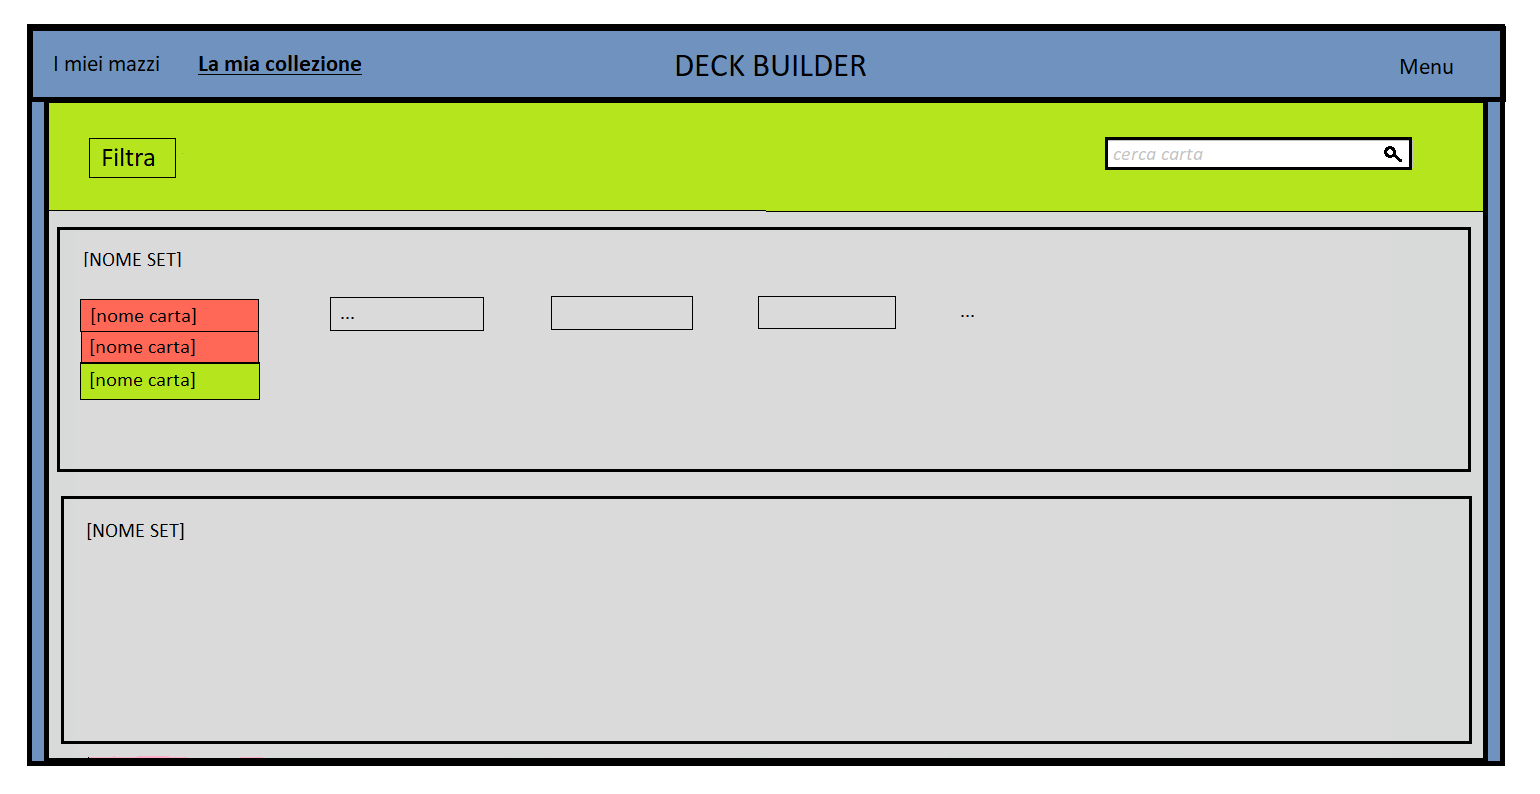
\includegraphics[width=13cm]{files/mockup_collezione.png}
    \caption{Pagina della collezione delle carte di un utente. Le carte sono divise per set, i cui nomi sono, all'atto pratico, sufficienti per distinguere tra i diversi CCG. All'interno del box di ogni set c'è la lista delle carte appartenenti ad esso, ciascuna contrassegnata in qualche modo come posseduta (sfondo verde) o mancante (sfondo rosso). E' possibile modificare la visualizzazione tramite il bottone "Filtra".}
    \label{fig:mockup_collezione}
\end{figure}
\begin{figure}[H]
    \centering
         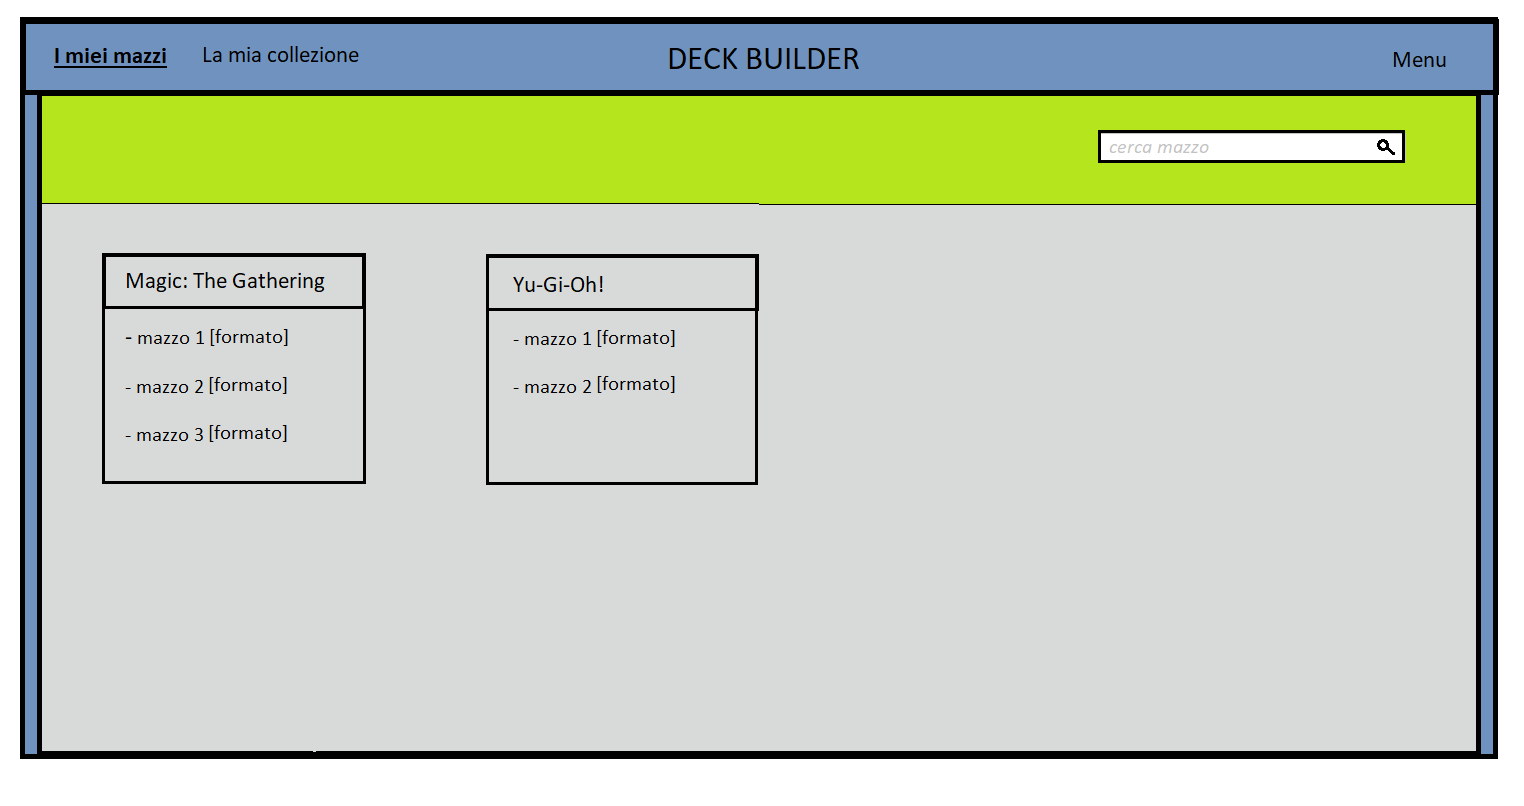
\includegraphics[width=13cm]{files/mockup_mazzi.png}
    \caption{Pagina dei mazzi, divisi per gioco, di un utente. Cliccando sul nome di un singolo mazzo si apre una schermata di visualizzazione e modifica dello stesso.}
    \label{fig:mockup_mazzi}
\end{figure}

\begin{figure}[H]
    \centering
         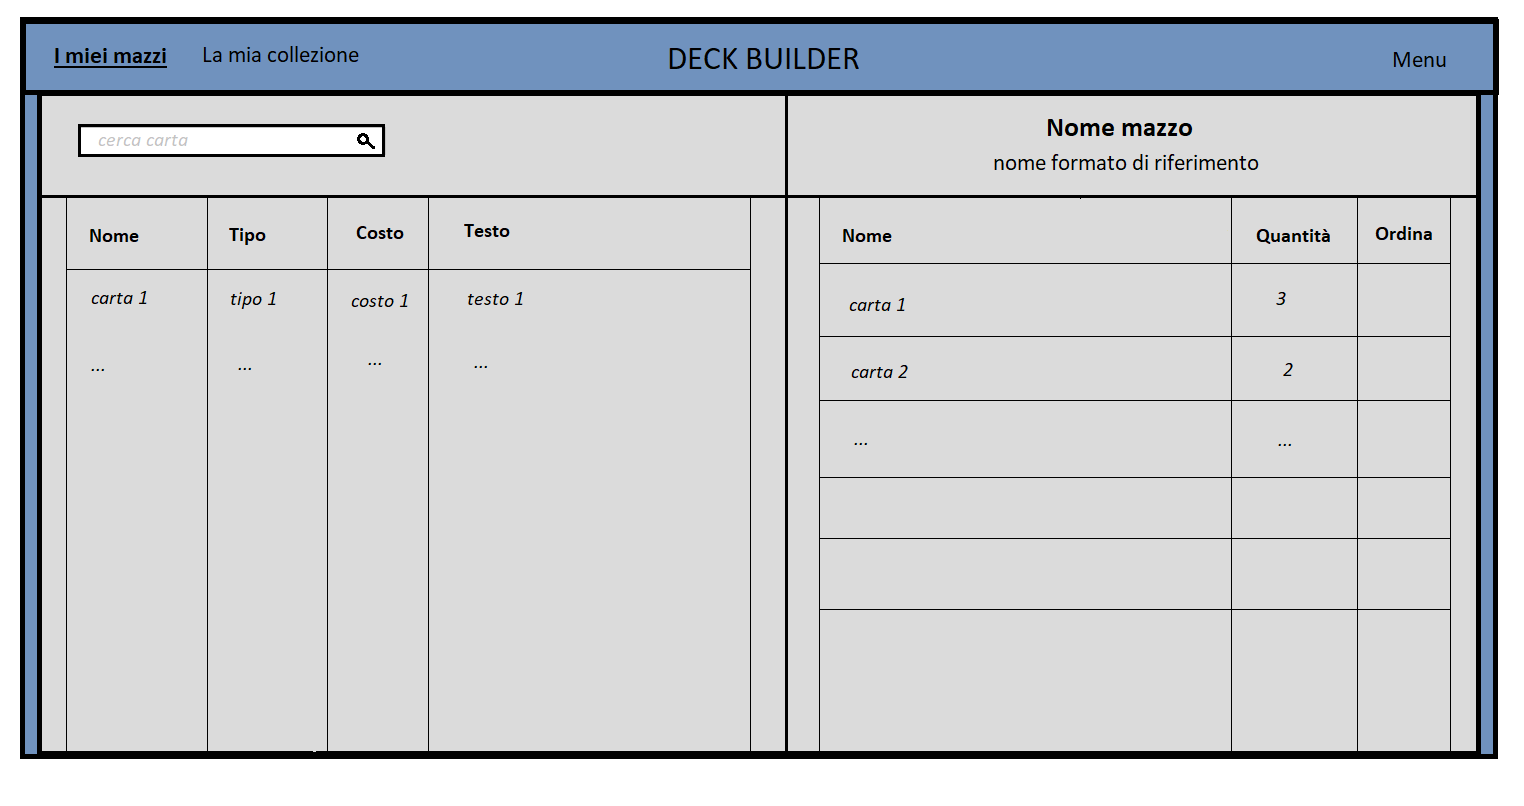
\includegraphics[width=13cm]{files/mockup_modifica_mazzo.png}
    \caption{Pagina della modifica di un mazzo. A sinistra abbiamo una sezione che permette di interrogare il database, mentre sulla destra la lista di carte che compongono il mazzo.}
    \label{fig:mockup_modifica_mazzo}
\end{figure}


\subsection{Task specifici e contesto}
I task principali che l'ontologia punta a rendere effettuabili sono:
\begin{itemize}
    \item fornire un meccanismo che permetta di tenere traccia delle carte in proprio possesso
    \item permettere la costruzione e la personalizzazione di un mazzo di carte
    \item permettere la ricerca di nuove carte potenzialmente interessanti sulla base di caratteristiche specifiche delle carte stesse
\end{itemize}

\subsection{Utenti target}
Gli utenti target sono di due tipi non esclusivi: i giocatori e i collezionisti. I primi potrebbero non aggiornare costantemente la loro collezione, ma utilizzare la piattaforma solamente per la gestione dei mazzi. Inoltre potrebbero non possedere fisicamente tutte le carte che inseriscono nei mazzi, ma averne delle proxy\footnote{In contesti amichevoli è d'uso non richiedere che ogni giocatore possieda una copia acquistata legalmente di ogni carta nel proprio mazzo, ma è sufficiente -dato il costo che possono raggiungere certe carte- averne una copia proxy, cioè stampata con la propria stampante. Questa pratica è spesso accettata anche dalle case produttrici stesse che, persino nei tornei convenzionati, permettono, sotto certe condizioni, l'uso di proxy. Si legga, per esempio, \url{https://magic.wizards.com/it/news/announcements/proxies-policy-and-communication-2016-01-14}}. I collezionisti, invece, porranno maggiore attenzione sulla propria collezione per vedere quali e quante siano le carte che ancora non possiedono.

\newpage
\section{Descrizione del Dominio e Fonti}
\subsection{Dominio}
\subsubsection{Introduzione}
Il mondo dei giochi di carte collezionabili vede il suo inizio nel 1993 con \textit{Magic: The Gathering}. Da allora molti altri giochi simili ad esso sono nati e hanno trovato, chi più chi meno, successo. In particolare con l’avvento dei giochi online alcuni si sono espansi o sono stati creati nativamente per vari dispositivi (PC, smartphone, ecc). C’è quindi al giorno d’oggi una grande diversità in questi giochi di carte, che però sono tutti accomunati da alcune caratteristiche chiave. \newline
In particolare un gioco di carte collezionabili tipicamente vede due persone, ciascuna dotata di un proprio mazzo, sfidarsi in un duello. Un duello è una partita organizzata in turni, la struttura dei quali esula dallo scopo di questa ontologia e pertanto non è qui riportata. Basti sapere che in generale durante il proprio turno un giocatore può giocare un qualsiasi numero di carte, con lo scopo ultimo di sconfiggere il proprio avversario.
Ogni giocatore inizia la partita con un numero fisso e uguale per tutti di punti vita. Questi possono essere ridotti in vari modi, e non appena un giocatore si trova ad avere 0 o meno punti vita, perde la partita. Un'altra condizione di sconfitta è il finire le carte nel proprio mazzo. \newline
Generalmente ogni CCG è associato a un universo narrativo, spesso di ambientazione fantastica, il quale rimane sotteso sia allo svolgimento di una partita che alle carte stesse, le quali ne traggono ispirazione per personaggi, eventi, o altro. Per esempio in \textit{Magic: The Gathering} i due giocatori sarebbero potenti maghi noti come "Planeswalker" che si sfidano a un duello evocando creature, scagliando magie o utilizzando artefatti dai poteri arcani.

\subsubsection{Mazzi e Formati}
Il Mazzo di ogni giocatore non ha una composizione predefinita come nei giochi di carte classici, ma è il proprietario che sceglie più o meno liberamente quali (e a volte anche quante) carte inserire nel proprio mazzo. Nel farlo deve tuttavia attenersi a delle regole di costruzione. Per esempio, in \textit{Magic: The Gathering} un mazzo non può contenere più di 4 copie di una stessa carta. \newline
Generalmente per ogni gioco possono esistere diversi Formati. Un Formato è sostanzialmente una serie di regole di costruzione di mazzi che può essere più o meno limitante delle regole generali. Per esempio nel formato \textit{Standard} di \textit{Magic: The Gathering} è possibile inserire una carta nel proprio mazzo solo se questa è sufficientemente recente, in particolare se è di uno degli ultimi 3 Set usciti (rimando al paragrafo \ref{p:set_espansioni} per una spiegazione di cosa siano i set). Al contrario, nel formato \textit{Commander} è invece permesso l'utilizzo di una qualsiasi carta a prescindere da quanto recente sia l'ultima ristampa (di nuovo, rimando a \ref{p:set_espansioni})  della stessa. \newline
Nel concreto, alcune Carte saranno permesse, o per meglio dire legali, in un certo Formato, mentre tutte le altre saranno illegali. Conseguentemente, anche un Mazzo sarà illegale in un certo Formato se contiene anche solo una Carta che a sua volta è illegale in quel Formato.


\subsubsection{Tipi di carte}
Le carte che compongono un mazzo sono di diversi tipi. Generalmente essi si suddividono in due categorie: "Permanenti" e "Non Permanenti". Le carte dei tipi appartenenti alla prima categoria permangono sul campo di gioco, e quindi continuano a influenzarlo, per un certo periodo di tempo dopo che sono state giocate. Le carte appartenenti ai tipi della seconda categoria, invece, hanno un effetto istantaneo e quindi vengono scartate subito dopo che sono state giocate.

I Permanenti si suddivono a loro volta in carte Unità, dotate di un attacco e una difesa, che possono attaccare l’avversario o le sue unità oppure bloccare gli attacchi delle unità avversarie, e carte Ausiliarie che invece non possono attaccare l'avversario ma avranno effetti genericamente utili. Un esempio sono le carte Equipaggiamento, da assegnare a un'unità per potenziarne le caratteristiche di attacco e difesa. 

Le carte Non Permanente invece si classificano in base alla velocità, cioè alla possibilità che ha l'avversario di rispondere all'effetto che avrebbe la carta giocata. A scopo meramente esemplificativo, in una situazione in cui un giocatore gioca una carta non permanente con velocità 2 che gli permetterebbe di distruggere un'unità dell'avversario, questi può giocare un'altra carta per salvare la sua unità solo se tale carta ha velocità maggiore di 2. Da notare che generalmente le regole che governano le possibilità di risposta a carte giocate dall'avversario sono molto più complesse di quanto possa far trasparire questo esempio. Inoltre le velocità stesse raramente si misurano con dei numeri, per esempio in \textit{Legends of Runeterra} ci sono 4 livelli di velocità che sono: "lento", "veloce", "concentrazione" e "raffica". \newline
Ai fini di questo progetto non è necessario rappresentare la velocità come una classe, ma è sufficiente averla come data property. Questa scelta di modellazione potrebbe, però, cambiare qualora lo scopo dell'ontologia fosse quello di portare alla costruzione di un programma che permetta di giocare una partita.

Ad ogni tipo di carta possono corrispondere uno o più possibili sottotipi. Questi sono soventemente subordinati ai tipi, e, nel caso delle carte non permanente potrebbero corrispondere ai livelli di velocità (non in tutti i CCG è così, però).
I sottotipi dipendono interamente dal gioco in esame, e pertanto le eventuali regole associate ad essi cambiano da gioco a gioco. Per questo motivo ho scelto di rappresentare anche i sottotipi come data property.

In ultimo, ogni carta è univocamente identificata (all'interno di un CCG) dal suo nome in lingua originale.


\subsubsection{Abilità delle carte}
Generalmente un giocatore vuole scegliere le carte da inserire nel proprio mazzo attenendosi a una tematica. Tale tematica influenzerà quindi sia il tipo di carte inserite nel mazzo che le abilità delle stesse. Ogni Carta può, infatti, avere una serie di Abilità, che le permettono di fare moltissime cose diverse. Le abilità vengono generalmente classificate in quattro categorie, ma non necessariamente un'abilità deve cadere in una di queste, proprio in virtù della grande diversità che le caratterizza. Talvolta un'abilità è anche in grado di modificare le regole stesse del gioco, e infatti vige sempre la cosiddetta "regola d'oro" dei CCG: il testo ufficiale di una carta ha sempre ragione. In ogni caso, le categorie sono: 
\begin{itemize}
    \item \textbf{Abilità Innescate:} sono abilità caratterizzate da una condizione e da una azione che verrà eseguita non appena si verifica la condizione, per esempio “All’inizio del turno, pesca una carta.”.
    \item  \textbf{Abilità Attivate:} sono abilità caratterizzate da un costo e da un’azione che viene eseguita quando un giocatore paga il costo. Per esempio “Scarta una carta per pescare una carta”.
    \item \textbf{Abilità Statiche:} sono abilità il cui effetto influenza continuamente il gioco. Per esempio “Le creature prendono +1/+1”, che implica che tutte le unità ottengano +1 all’attacco e +1 alla difesa.
    \item \textbf{Abilità Parole Chiave} o \textbf{Keyword:} sono abilità definite da una parola chiave, alla quale è associato un testo esteso generalmente contenuto nel manuale di regole del gioco stesso. Per esempio, in \textit{Magic: The Gathering} la keyword “Difensore” è associata al testo esteso “Questa creatura non può attaccare”.
\end{itemize}

 In utlimo, le abilità possono far riferimento a carte specifiche. In questo caso diremo che la carta che possiede tale abilità \textit{interagisce con} la carta nominata.

\subsubsection{Rarità delle carte}
Le carte sono inoltre divise da un sistema di rarità, dove alle carte con abilità più forti corrisponderà una rarità maggiore, e a quelle con abilità più deboli invece una rarità minore. La rarità di una carta influenza anche la probabilità di trovarla in una bustina (rimando al paragrafo \ref{p:set_espansioni}).

\subsubsection{Risorse}
Ogni gioco utilizza un sistema di risorse, paragonabili a una moneta di gioco che viene utilizzata principalmente per pagare dei Costi. Pagare un Costo è una condizione necessarie per effettuare varie azioni nell’arco di una partita. La prima, nonché più importante, è il giocare le carte stesse. Ogni carta, infatti, può avere un Costo in termini di risorse di gioco che sarà tanto più alto quanto più forte è la carta (in maniera simile alla rarità, ma indipendente da essa). Una seconda azione possibile pagando un Costo è attivare un'Abilità Attivata.\newline
Le risorse possono essere di diverso tipo e di diversa origine. Possono infatti essere generate automaticamente per i giocatori, oppure richiedere alcune carte specifiche. Per esempio nel gioco \textit{Legends of Runeterra} ogni giocatore all’inizio del turno riceve un numero crescente di mana, l’unica risorsa del gioco, senza che egli debba intraprendere alcuna azione particolare. In \textit{Magic: The Gathering}, invece, i diversi tipi di risorsa devono essere attinti da altrettanti sottotipi di carta che fanno riferimento al tipo di carta chiamato "Terra". Per esempio il tipo di risorsa "Mana blu" potrà essere attinto solamente dalle Terre del sottotipo "Isola". \'E quindi evidente come, a seconda del gioco, la composizione del mazzo potrebbe dover tenere in considerazione anche aspetti legati alla produzione di risorse che potrebbero servire nel corso di una partita.

\subsubsection{Set, espansioni e commercializzazione}
\label{p:set_espansioni}
Altra particolarità dei giochi di carte collezionabili riguarda il come essi vengano commercializzati. In particolare, le carte vengono vendute (in diversi prodotti) sulla base dei blocchi, a loro volta divisi in set. Un set è un insieme di carte accomunate, generalmente, da un arco narrativo ambientato nell’universo di riferimento del gioco oppure da una tematica generale. Per esempio, l’ultima espansione di Magic: The Gathering è chiamata “Phyrexia: All Will Be One” e le carte in essa sono legate al tentativo della fazione di Phyrexia (arcinemico nell’universo narrativo di MTG) di conquistare l’intero Multiverso. Ogni set può introdurre carte nuove oltre che ristampare carte già esistenti. Queste ultime sono dette "ristampe". Un blocco non è altro che una serie di set ambientati nello stesso arco narrativo. Le differenze esatte tra Set e Blocchi variano da gioco a gioco, tanto che i blocchi non sempre esistono. \newline
Come accennato poc’anzi, per ogni Set esistono prodotti di vario tipo. Esistono mazzi precostruiti di cui è nota la lista di carte, oppure bustine “a scatola chiusa” di cui si sa solamente la composizione generale. Anche qui, ogni gioco ha ampia libertà di manovra. In ogni caso questa ontologia non si occupa dei prodotti relativi ai giochi, ma solamente di a quale Set appartenga una carta, in modo da distinguere le eventuali ristampe per gli utenti collezionisti.

\subsection{Fonti}
Per la modellazione del dominio mi sono basato, oltre che su specifiche sezioni degli articoli già menzionati in precedenza, sulle pagine Wikipedia in inglese\footnote{Wikipedia: Collectible Card Game \url{https://en.wikipedia.org/wiki/Collectible_card_game}} e in italiano\footnote{Wikipedia: Giochi di carte collezionabili \url{https://it.wikipedia.org/wiki/Gioco_di_carte_collezionabili}} relative ai CCG, sul libro “Trading Card Games for Dummies”\footnote{Trading Card Games for Dummies, John Kaufeld, Jeremy Smith; pubblicato da Wiley Publishing Inc; ISBN-13: 978-0-471-75416-9}. In ultimo, mi sono basato anche sulla mia esperienza personale da giocatore di alcuni tra i CCG più conosciuti (Yu-Gi-Oh!, Magic: The Gathering, Pokemon, ecc).
\newpage


\section{Documentazione del Dominio}
\subsection{Risorse simili ed ispirazione}

Per la costruzione di questa ontologia mi sono basato su varie piattaforme già esistenti dal funzionamento simile. Prima tra tutte \url{http://www.scryfall.com/advanced}, per la funzione di ricerca di carte. Scryfall in particolare si occupa solamente delle carte di \textit{Magic: The Gathering} e proprio per questo ha molti filtri specifici delle carte di MTG come "Colors" (Colori) e altri. La forza di scryfall è che, oltre all'interfaccia presentata in Figura \ref{fig:scryfall}, permette l'interrogazione del DB anche tramite un linguaggio di query apposito, di cui si possono conoscere i dettagli cliccando sul bottone "Syntax" che si trova in alto a destra nell'immagine. Mostriamo quindi una query di esempio, con relativi risultati, in Figura \ref{fig:scryfall_query}.

\begin{figure}[H]
    \centering
         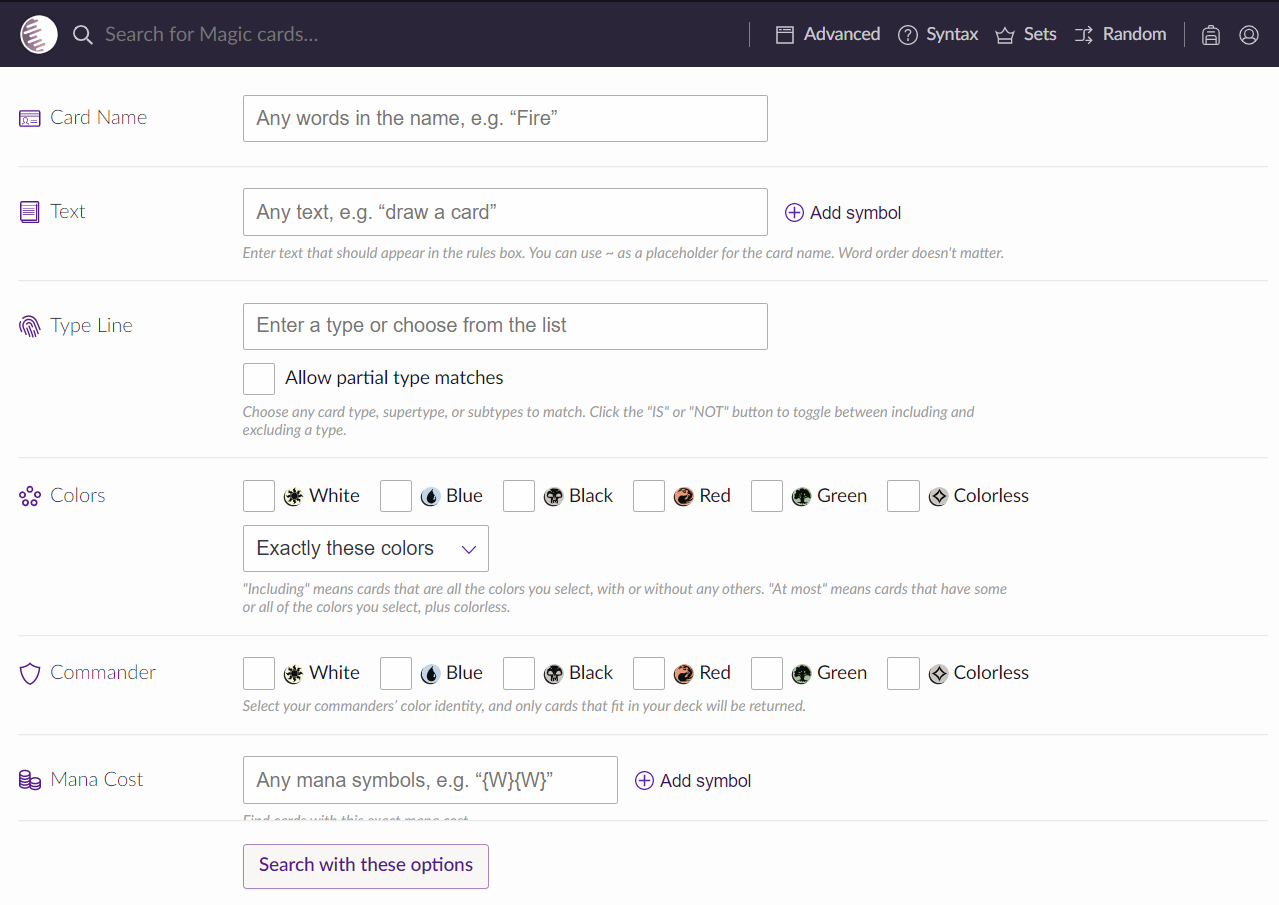
\includegraphics[width=14cm]{files/scryfall_advanced.png}
    \caption{Ricerca avanzata di scryfall.com}
    \label{fig:scryfall}
\end{figure}

\begin{figure}[H]
    \centering
         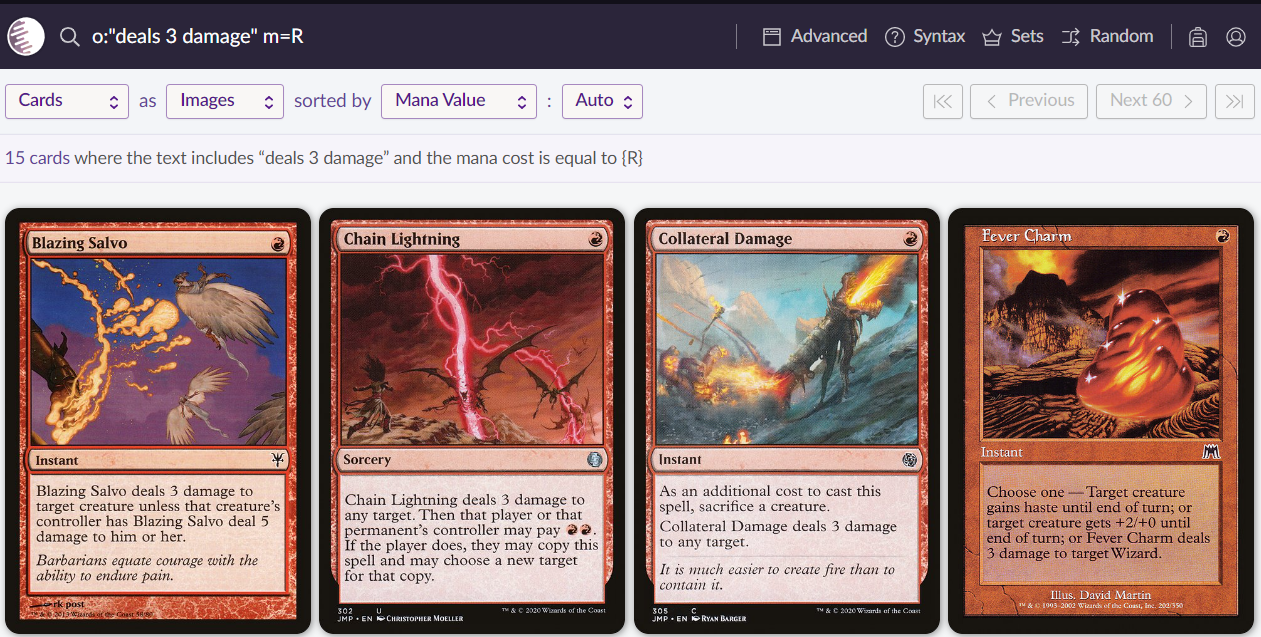
\includegraphics[width=14cm]{files/scryfall_query.png}
    \caption{Esempio di query su scryfall.com. Si cercano tutte le carte che hanno "deals 3 damage" nel testo e hanno costo pari a un mana rosso. Sono mostrati solo i primi 4 risultati.}
    \label{fig:scryfall_query}
\end{figure}

\begin{figure}[H] 
    \centering
         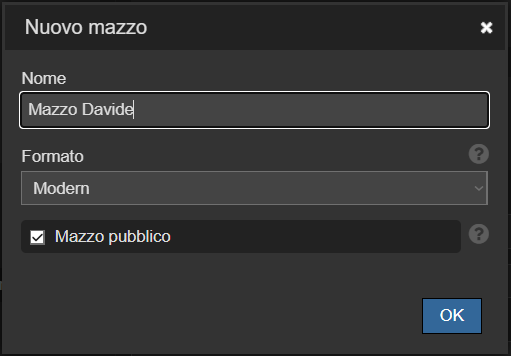
\includegraphics{files/deckstats_1.png}
    \caption{Popup di creazione del mazzo in deckstats.net}
    \label{fig:deckstats_1}
\end{figure}


L'idea iniziale che ha poi portato alla costruzione di questa ontologia era infatti costruire una piattaforma che, similmente a scryfall, permettesse l'interrogazione di un db tramite un linguaggio di query unificato per ogni CCG. Tuttavia l'ontologia effettiva è poi evoluta in quanto già descritto nei capitoli precedenti.

La seconda piattaforma a cui mi sono ispirato è \url{http://www.deckstats.net/}, che permette agevolmente di creare e modificare mazzi, impostandoli come validi per uno specifico formato, oppure etichettandoli come "Casual", cioè che non fanno riferimento ad uno specifico formato, ma verranno utilizzati per giocare con amici. Deckstat è anche in grado di segnalare automaticamente all'utente se il mazzo che ha costruito sia effettivamente legale nel formato per cui è stato pensato oppure no. In Figura \ref{fig:deckstats_1} vediamo la finestra popup di creazione di un mazzo, all'interno della quale sono da inserirne il nome e il formato di riferimento. In Figura \ref{fig:deckstats_2}, invece, vediamo la schermata di modifica di un mazzo che è divisa in due sezioni: a sinistra la sezione database da cui è possibile cercare le carte impostando vari filtri tramite interfaccia grafica, mentre a destra abbiamo la lista di carte che compongono il mazzo, ciascuna con la propria quantità.

\begin{figure}[H]
    \centering
         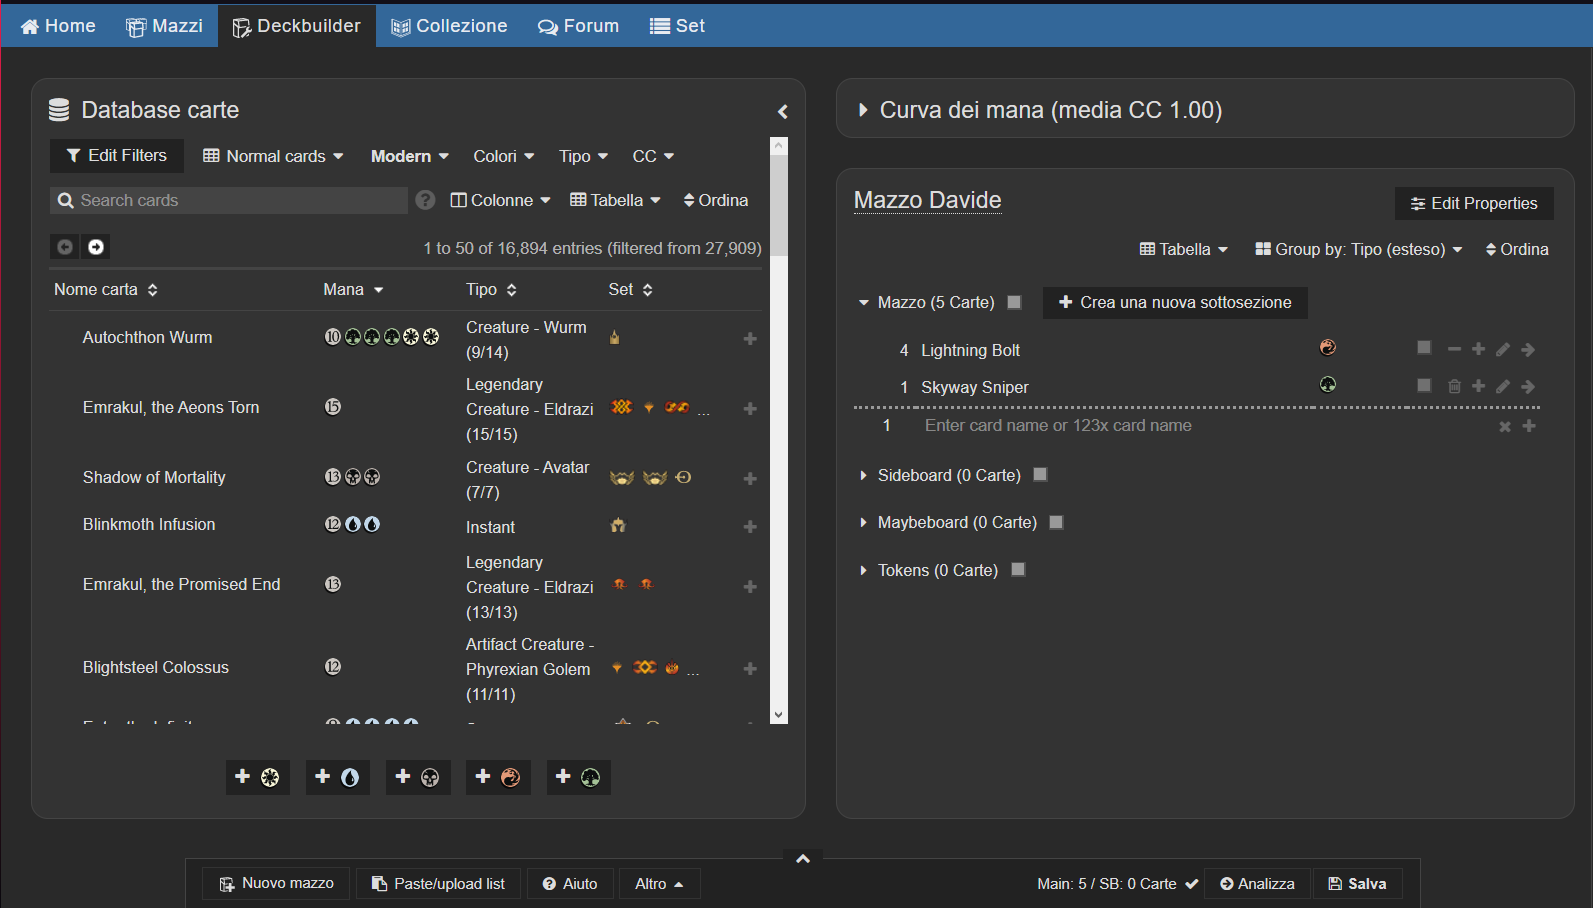
\includegraphics[width=14cm]{files/deckstats_2.png}
    \caption{Schermata di modifica del mazzo in deckstats.net}
    \label{fig:deckstats_2}
\end{figure}

L'obiettivo per l'ipotetica piattaforma sviluppata a partire da questa ontologia, almeno per quanto riguarda gli utenti giocatori, sarebbe quello di integrare i due punti di forza di queste piattaforme e permettere la ricerca delle carte tramite un linguaggio di query strutturato e facilmente comprensibile dai giocatori, direttamente dalla schermata di modifica del mazzo, in modo da facilitare la ricerca di nuove carte da inserirvi.

Per quanto riguarda gli utenti collezionisti, invece, vediamo, sempre da Deckstats, la pagina relativa a "La mia collezione" in Figura \ref{fig:deckstats_3}.

\begin{figure}[H]
    \centering
         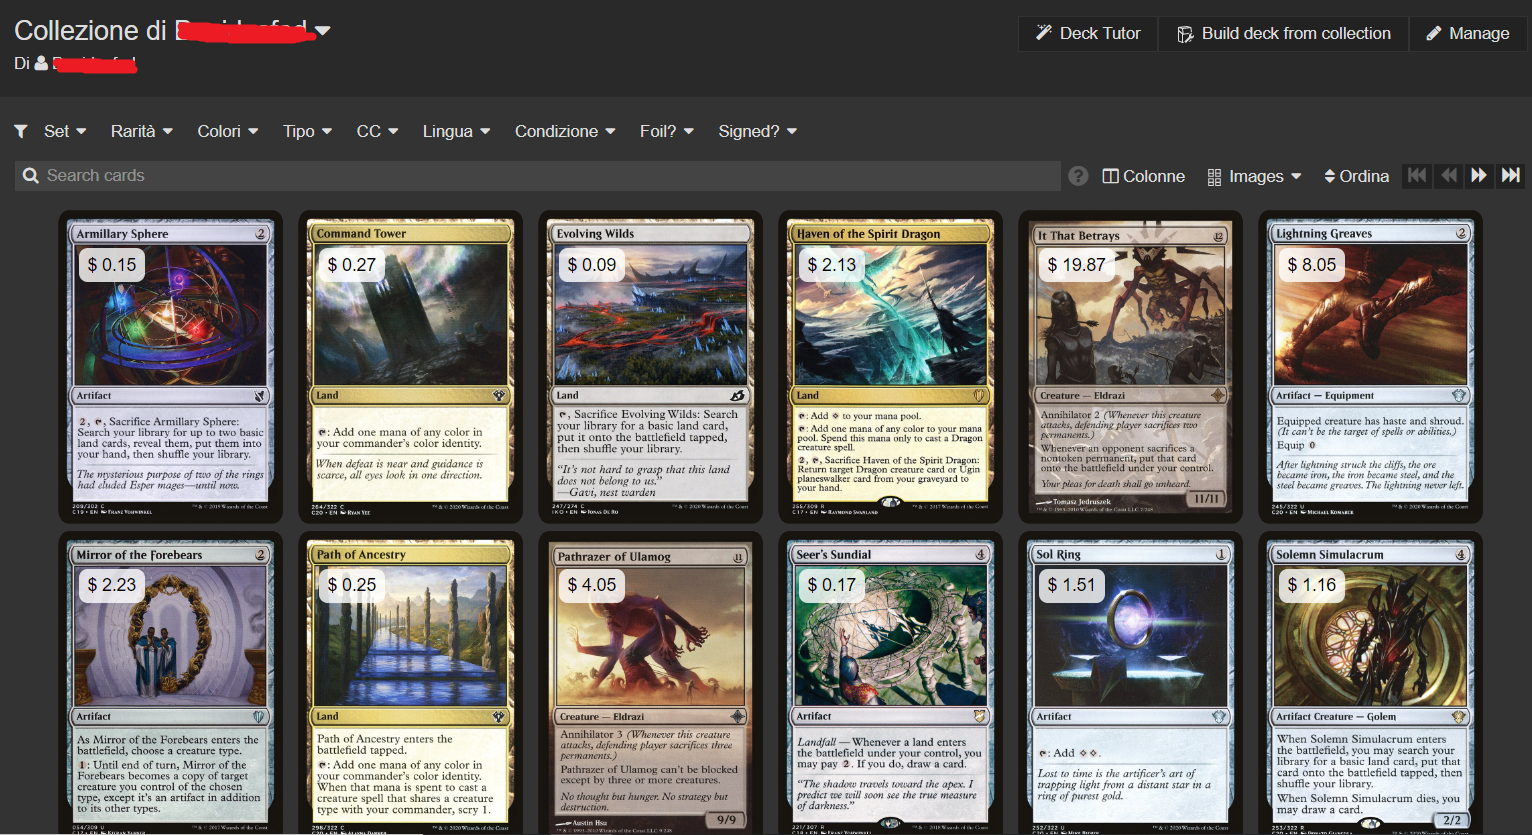
\includegraphics[width=14cm]{files/deckstats_3.png}
    \caption{Pagina "La mia collezione" in deckstats.net. Il nome utente è stato coperto per ragioni di privacy.}
    \label{fig:deckstats_3}
\end{figure}

Come si può vedere, la collezione è composta da un'accozzaglia di carte, inizialmente non divise in alcun modo. L'idea per l'ipotetica applicazione derivante da questa ontologia, come già mostrato nei mockup in Figura \ref{fig:mockup_collezione}, sarebbe non far comparire direttamente la carte, ma  una lista dei vari set, evidenziando in qualche maniera quelli completi, in modo che il collezionista abbia un colpo d'occhio più adatto alle sue esigenze rispetto a quello fornito da Deckstats. Futuri sviluppi della piattaforma potrebbero essere anche quelli di permettere al collezionista stesso di creare dei set personalizzati.


A questo punto non rimane che da analizzare la visualizzazione delle singole carte. Per questo particolare obiettivo ho preso come ispirazione la piattaforma \url{http://www.https://app.mobalytics.gg/}, che si occupa, tra le altre cose, del CCG online \textit{Legends of Runeterra}. \newline
La forza di mobalytics sta nel fatto che permette una navigazione immediata dei legami tra le singole carte. In Figura \ref{fig:carte_vayne} si vede che sotto Vayne ci sono 4 pallini, ciascuno che simboleggia una carta con cui Vayne interagisce. Ci sarà, per esempio, la carta Tumble, che può essere creata da Vayne a ogni inizio del turno. In generale una carta potrebbe interagire con molte altre carte, e quindi è utile avere un meccanismo immediato che permetta, partendo da essa, di raggiungere facilmente tutte le altre senza dover effettuare un'altra query.
Oltre a ciò possiamo notare che mobalytics, a destra della carta, mantiene tutte le informazioni della carta stessa quali le abilità, l'attacco e la difesa, i tipi e i sottotipi, ecc.

\begin{figure}[H]
    \centering
         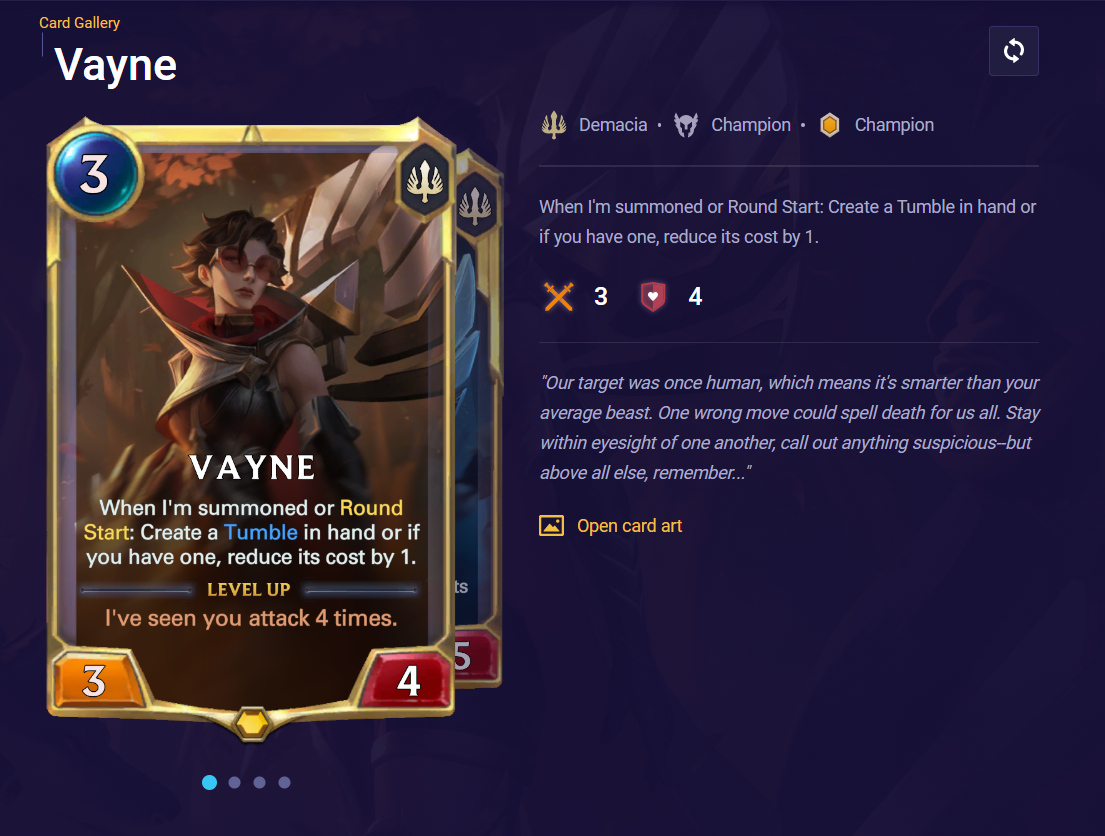
\includegraphics[width=13cm]{files/carte_vayne.png}
    \caption{Pagina relativa alla carta "Vayne" in mobalytics.org, al link \url{https://app.mobalytics.gg/lor/cards/06DE021}}
    \label{fig:carte_vayne}
\end{figure}



\subsection{Allineamenti}
Per quanto riguarda gli allineamenti con altre risorse, si è scelto di utilizzare DBpedia e FOAF. L'allineamento con DBpedia è risultato sostanzialmente forzato in quanto è l'unica risorsa esterna che io abbia trovato che aveva qualche legame con i CCG che potesse essere utile con riferimento alle finalità espresse nella sezione dedicata di questo documento. Sebbene esista un certo numero di ontologie dedicate all'ambito dei giochi, infatti, molte si concentrano più sulla loro classificazione o sull'effettivo svolgimento di una partita, obiettivi che poco o nulla hanno a che vedere con quelli attuali di ccgo. \newline
L'allineamento con foaf, invece, risulta utile se si pensa che un futura possibile espansione di ccgo potrebbe essere l'inserimento di feature tipiche dei social network, quali per esempio la possibilità di relazioni tra i Giocatori che potrebbero permettere lo scambio di idee per i mazzi.

In ogni caso, nella seguente tabella presentiamo le principali corrispondenze.

\begin{center}
\begin{tabular}{ |c|c|c| } 
 \hline
CCGO & PROPRIET\'A & RISORSA \\
 \hline
 GiocoCarteCollezionabili & owl:equivalentTo & \href{http://dbpedia.org/resource/Collectible_card_game}{dbr:Collectible\_card\_game} \\ 
 
 Carta & rdfs:subclassOf & \href{http://dbpedia.org/resource/Playing_card}{dbr:Playing\_card} \\ 
 
 Giocatore & rdfs:subclassOf & \href{http://dbpedia.prg/resource/Player_(cards)}{dbr:Player\_(cards)} \\ 
 
 Collezionista & skos:related & \href{http://dbpedia.org/resource/Category:Collectors}{dbc:Collectors} \\

 Mazzo & skos:related & \href{http://dbpedia.org/resource/Deck_(cards)}{dbr:Deck\_(cards)} \\

 Persona & rdfs:subclassOf & \href{http://xmlns.com/foaf/0.1/#Person}{foaf:Person} \\
 \hline
\end{tabular}
\end{center}

Alcune note su queste corrispondenze:
\begin{itemize}
    \item L'IRI dbr:Deck\_(cards) rimanda alla risorsa dbr:Playing\_card, già allineata con la classe Carta. Ciò giustifica la relazione skos:related.
    \item per le classi Carta, Giocatore e Collezionista si consideri che in ccgo ci si limita strettamente all'ambito dei CCG, escludendo quindi, per esempio, le carte da gioco classiche. Ciò giustifica le relazioni skos:related e rdfs:subclassOf. Nello specifico, per Collezionista si è seguito una scelta contenuta in dbpedia stessa. Infatti dbc:Collectors è skos:related con dbc:Song\_collectors e dbc:Plant\_collectors. Risulta quindi sensato supporre che un'eventuale risorsa dbc:CCG\_collectors (che sarebbe stata equivalente a Collezionista) dovrebbe seguire il medesimo pattern.
\end{itemize}


\subsection{Ontology Design Pattern}
Per quanto riguarda gli ODP scelti, invece, poiché le classi Mazzo e Collezione sono insiemi di carte dove il numero di copie di ogni singola carta è importante, si è deciso di utilizzare \href{http://ontologydesignpatterns.org/wiki/Submissions:Bag}{Bag}.
In Figura \ref{fig:bag} una rappresentazione delle classi di Bag. In particolare, come si vede dalla tassonomia di ccgo contenuta nella sezione successiva, le classi Bag e Item sono state espanse con delle classi ad hoc, così come le proprietà itemContent e itemOf/hasItem.

\begin{figure}[H]
    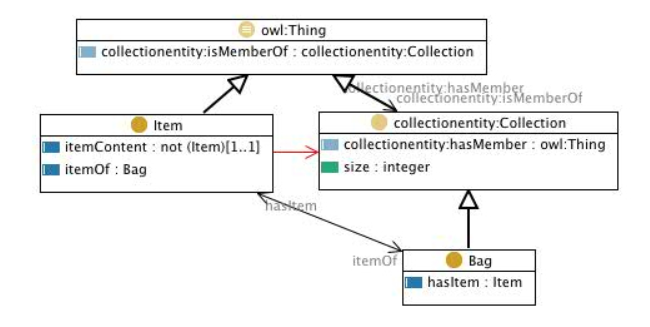
\includegraphics[width=14cm]{files/bag.png}
    \caption{Schema di Bag}
    \label{fig:bag}
\end{figure}

\newpage
\section{Visualizzazione Ontologia}

Iniziamo con il visualizzare la tassonomia dell'ontologia al completo.

\begin{figure}[H]
    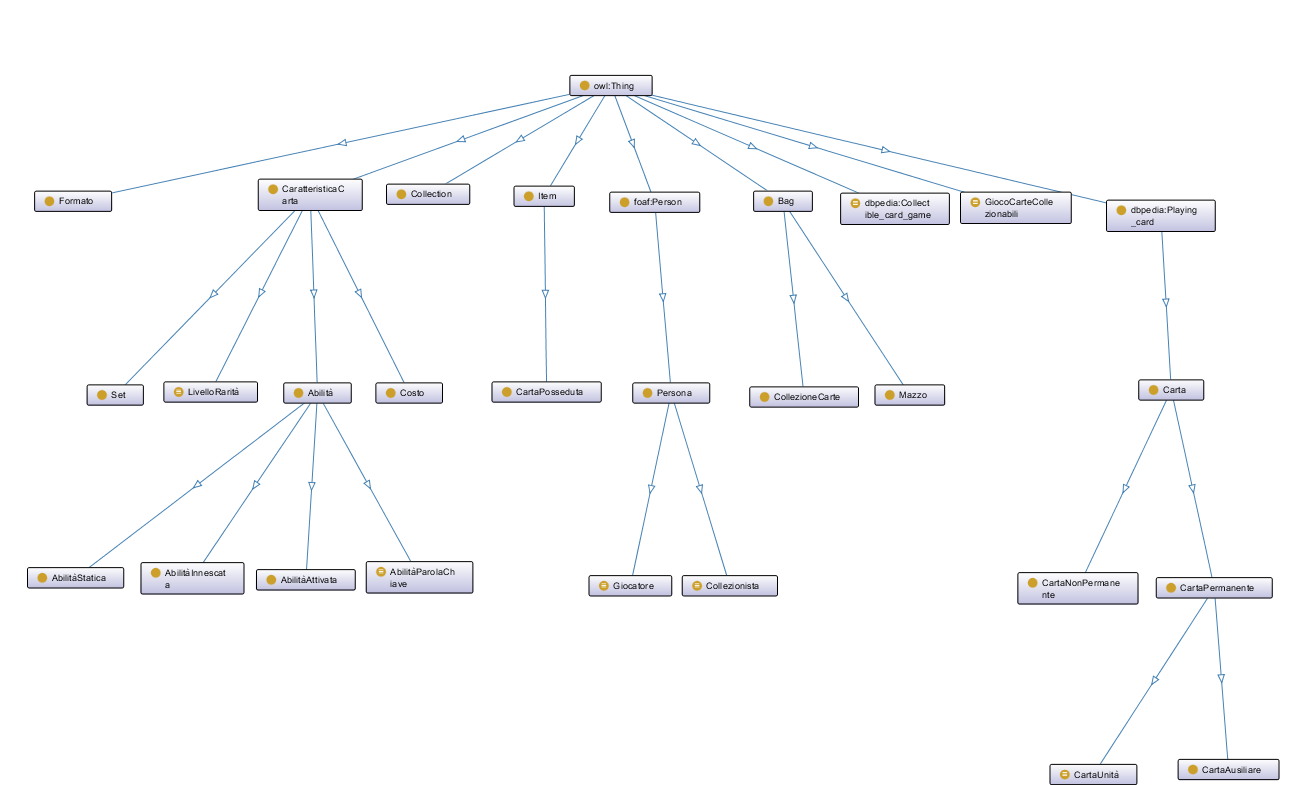
\includegraphics[width=14cm]{files/tassonomia.png}
    \caption{Tassonomia di ccgo}
    \label{fig:tassonomia}
\end{figure}

Una versione di maggiori dimensioni di questa immagine è disponibile nel repository github.

Passiamo quindi a dedicarci ad alcune entità.
La prima, nonché più importante, è la classe Carta. Come esempio prendiamo la carta di MTG chiamata "Ornitottero". In Figure \ref{fig:triple_ornitottero_1} e \ref{fig:triple_ornitottero_2} vediamo le triple che la definiscono, prese da GraphDB. In Figura \ref{fig:grafo_ornitottero} vediamo anche il visual graph associato (non tutte le triple sono presenti).

\begin{figure}[H]
    \centering
    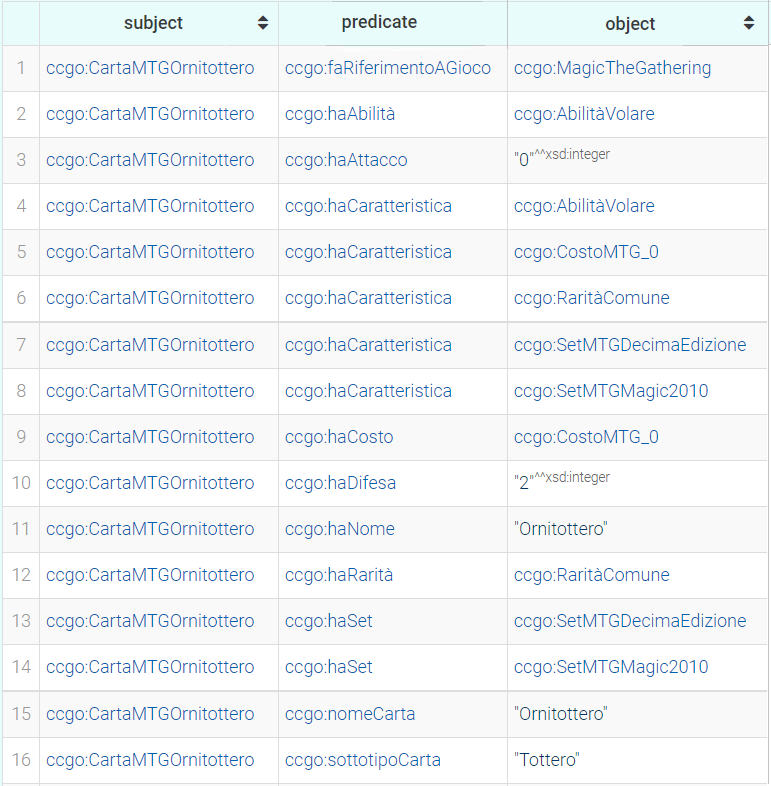
\includegraphics[width=14cm]{files/triple_ornitottero.png}
    \caption{Triple rdf relativa alla carta "Ornitottero" di Magic the Gathering}
    \label{fig:triple_ornitottero_1}
\end{figure}
\begin{figure}[H]
    \centering
    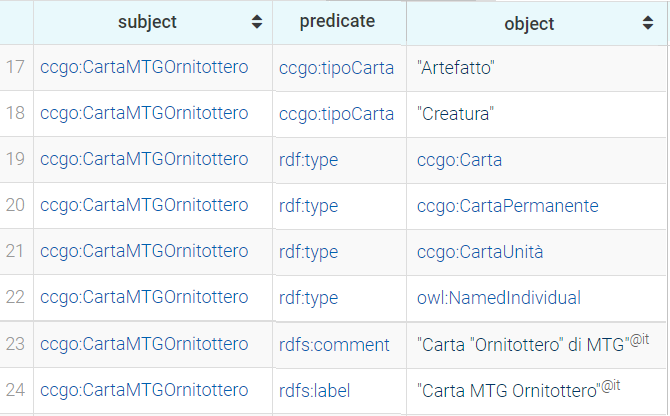
\includegraphics[height=7.5cm]{files/triple_ornitottero_2.png}
    \caption{Triple rdf relativa alla carta "Ornitottero" di Magic the Gathering}
    \label{fig:triple_ornitottero_2}
\end{figure}

\begin{figure}[H]
    \centering
    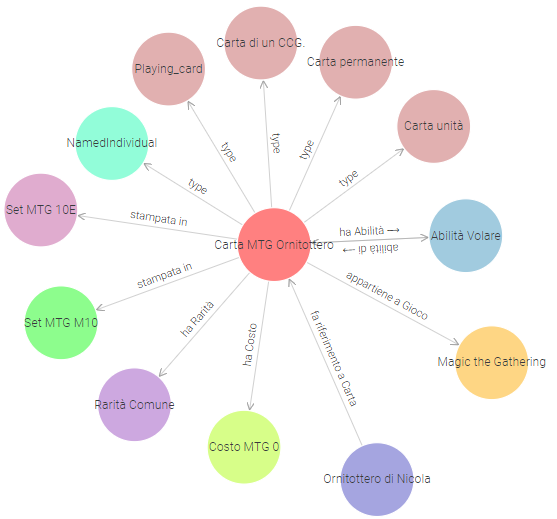
\includegraphics[height=9cm]{files/grafo_ornitottero.png}
    \caption{Visual graph della carta "Ornitottero"}
    \label{fig:grafo_ornitottero}
\end{figure}

In secondo luogo per quanto riguarda i Mazzi e le Collezioni, dal momento che i due casi sono molto simili presentiamo solamente il Mazzo "RossoVerde". Da notare che questo mazzo di esempio è composto solamente da 4 copie di una singola carta. Questo è dovuto alla semplicità di rappresentazione necessaria in un esempio. All'atto pratico un mazzo di Magic deve contenere, nel migliore dei casi, almeno 40 carte contando anche le copie. Numeri simili sono utilizzati anche da molti altri CCG.

\begin{figure}[H]
    \centering
    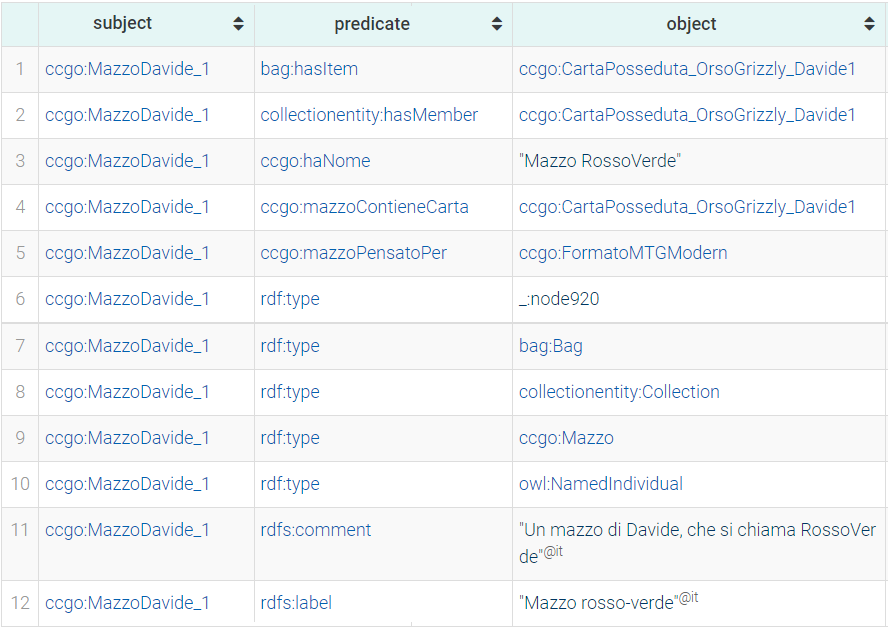
\includegraphics[width=13cm]{files/triple_mazzo.png}
    \caption{Triple rdf relativa al Mazzo RossoVerde}
    \label{fig:triple_mazzo}
\end{figure}

\begin{figure}[H]
    \centering
    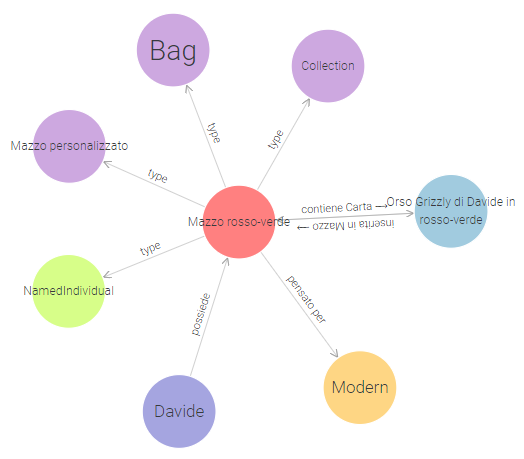
\includegraphics[height=9cm]{files/grafo_mazzo.png}
    \caption{Visual graph del Mazzo Rosso-Verde}
    \label{fig:grafo_mazzo}
\end{figure}




\newpage
\section{Interazioni con l'utente}
In questa sezione analizziamo alcuni pattern di interazione che ci aspettiamo ccgo possa avere. \'E tuttavia doveroso fare prima alcune premesse.

I dati di esempio mostrati nelle query sono tutti riferiti al gioco \textit{Magic: The Gathering}, in quanto questo è il più conosciuto (nonché il primo storicamente) tra i CCG. Inoltre le query qui presentate, con relativi risultati, sono screenshot presi da GraphDB, ed in ognuna di esse diamo per scontato di utilizzare i seguenti prefissi.
\begin{figure}[H]
    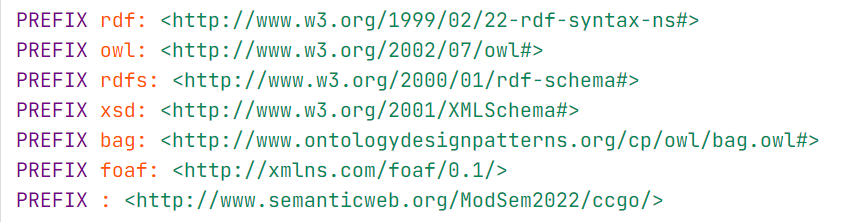
\includegraphics[width=14cm]{files/prefissi_query.png}
    \caption{Prefissi delle query}
    \label{fig:prefissi_query}
\end{figure}

I titoli delle seguenti sezioni sono sintesi dell'interazione stessa, che sarà spiegata in dettaglio all'interno della sezione.

\subsection{Giocatore modifica mazzo}
La prima interazione che analizziamo è quella tra il sistema e un utente giocatore, che chiameremo Davide. Egli desidera modificare un mazzo per il quale ha ottenuto recentemente nuove carte, e pertanto accederà anzitutto alla lista dei suoi mazzi, per poi selezionare quello di suo interesse e modificarlo.

\begin{figure}[H]
    \centering
    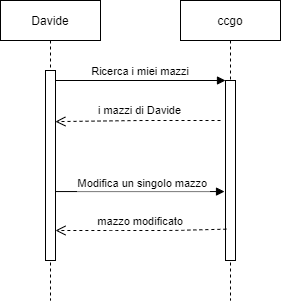
\includegraphics[height=8cm]{files/flowchart_davide.png}
    \caption{Diagramma d'interazione per l'utente giocatore}
    \label{fig:flowchart_davide}
\end{figure}

In Figura \ref{fig:query1_davide} vediamo la richiesta della lista dei mazzi appartenenti a Davide, ciascuno con il propro nome.

\begin{figure}[H]
    \centering
    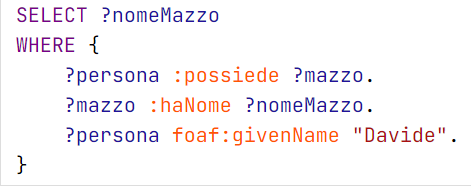
\includegraphics[]{files/query1_davide.png}
    \caption{Query di ricerca dei mazzi di Davide}
    \label{fig:query1_davide}
\end{figure}

Da notare che la seguente query restituisce unicamente dei Mazzi solo se le collezione di carte di Davide è senza nome, cosa che, nell'uso ideale di questo sistema, dovrebbe essere garantito. In alternativa, è necessario aggiungere una clausola \mintinline{SPARQL}{?mazzo rdf:type :Mazzo} alla query.

Come vediamo in Figura \ref{fig:res1_davide} la risposta  contiene due mazzi.

\begin{figure}[H]
    \centering
    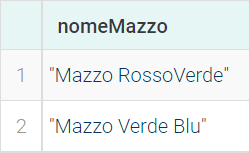
\includegraphics[]{files/res1_davide.png}
    \caption{I mazzi di Davide}
    \label{fig:res1_davide}
\end{figure}

A questo punto l'utente ne selezionerà uno, supponiamo il mazzo "RossoVerde". La prossima query, in  Figura \ref{fig:query2_davide}, si occupa quindi di visualizzare la lista delle carte che compongono tale mazzo. La risposta è mostrata in Figura \ref{fig:res2_davide}.

\begin{figure}[H]
    \centering
    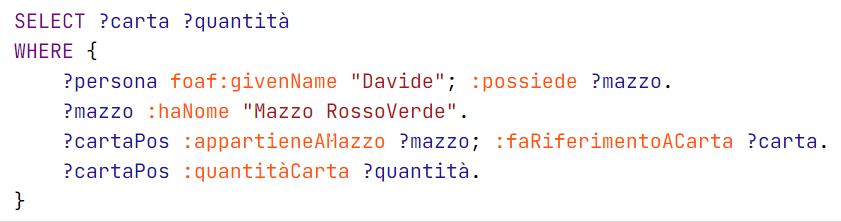
\includegraphics[width=14cm]{files/query2_davide.png}
    \caption{Query di ricerca delle carte che compongono il mazzo "RossoVerde" di Davide}
    \label{fig:query2_davide}
\end{figure}

\begin{figure}[H]
    \centering
    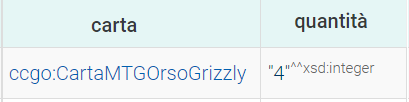
\includegraphics[]{files/res2_davide.png}
    \caption{Lista delle carte nel mazzo RossoVerde}
    \label{fig:res2_davide}
\end{figure}

Da notare che questa query può dare dei risultati non intuitivi qualora Davide abbia inserito più copie della stessa carta appartenenti a Set diversi. L'assunzione di fondo è che delle carte inserite in un mazzo non sia importante mantenere anche l'informazione riguardante il set, pertanto questa eventualità non dovrebbe verificarsi.

Riprendendo il flusso di interazione, Davide a questo punto può inserire le nuove carte. In particolare supponiamo che sia entrato in possesso della carta "Fulmine" di \textit{Magic: The Gathering} e che quindi voglia aggiungerne 3 copie al mazzo "RossoVerde". La query di inserimento è riportata in Figura \ref{fig:query3_davide}

\begin{figure}[H]
    \centering
    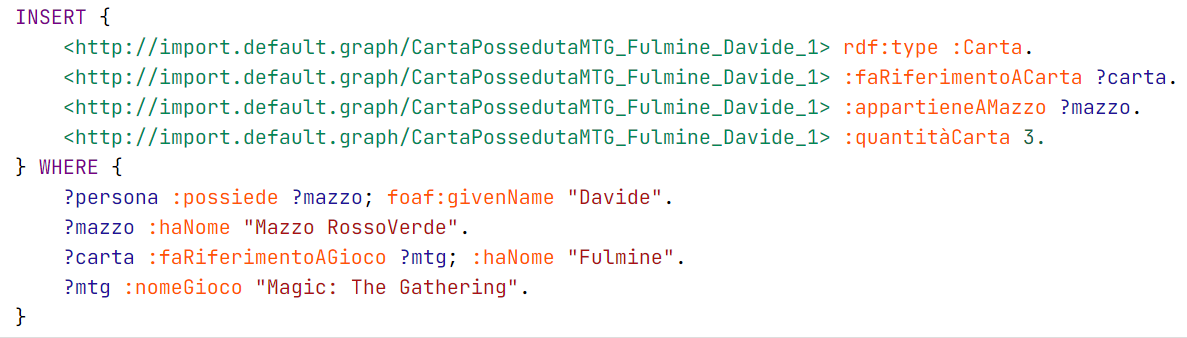
\includegraphics[width=14cm]{files/query3_davide.png}
    \caption{Query di inserimento della carta "Fulmine" nel mazzo "RossoVerde" di Davide}
    \label{fig:query3_davide}
\end{figure}

Si noti che non è specificato a quale Set appartenga la carta Fulmine inserita. Questo va a sostegno di quanto detto prima.\newline
Per vedere il risultato di questa query ripetiamo la query mostrata in Figura \ref{fig:query2_davide} in modo da vedere che effettivamente la carta Fulmine è stata aggiunta al mazzo.

\begin{figure}[H]
    \centering
    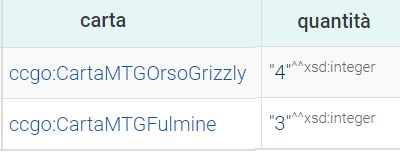
\includegraphics[]{files/res3_davide.png}
    \caption{Lista delle carte nel mazzo RossoVerde}
    \label{fig:res3_davide}
\end{figure}

\subsection{Giocatore cerca carta}
Come seconda interazione, supponiamo ora che un giocatore, sempre Davide, voglia modificare un proprio mazzo la cui tematica siano le creature dotate della parola chiave "Volare". Supponiamo inoltre che Davide voglia cercare nuove carte da acquistare per poi inserirle nel proprio mazzo. Per fare questo dovrà prima accedere alla lista delle carte che compongono il mazzo che vuole modificare, per poi ricercare tutte le carte di \textit{Magic: The Gathering} che abbiano le seguenti caratteristiche:
\begin{itemize}
    \item deve avere il tipo di carta "Creatura"
    \item deve avere l'abilità parola chiave "Volare"
\end{itemize}

Infine dovrà aggiungere le carte selezionate al proprio mazzo.
Qui di seguito mostriamo il flowchart di questa interazione.

\begin{figure}[H]
    \centering
    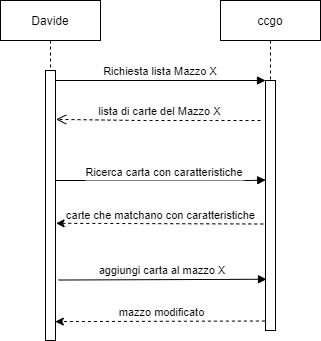
\includegraphics[height=9cm]{files/flowchart_davide_ricerca_carta.png}
    \caption{Diagramma d'interazione per l'utente giocatore}
    \label{fig:flowchart_davide_ric_carta}
\end{figure}

Il primo e terzo step di questa interazione sono analoghi a quanto già visto nelle query mostrate rispettivamente in Figura \ref{fig:query1_davide} e \ref{fig:query3_davide}. Passiamo quindi direttamente alla ricerca delle carte che matchano con le caratteristiche descritte sopra.

\begin{figure}[H]
    \centering
    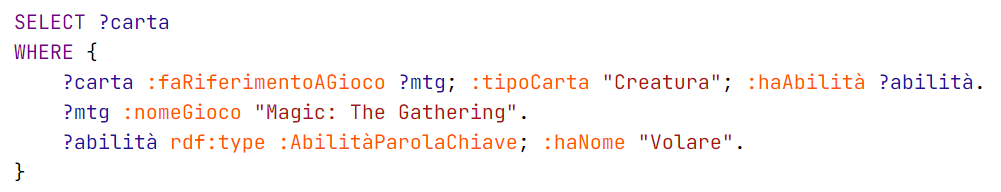
\includegraphics[width=14cm]{files/query4_davide.png}
    \caption{Query di ricerca di carte Creatura con l'abilità Volare}
    \label{fig:query4_davide}
\end{figure}

\begin{figure}[H]
    \centering
    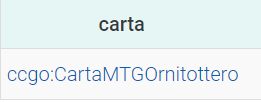
\includegraphics[]{files/res4_davide.png}
    \caption{Lista delle carte Creatura con Volare}
    \label{fig:res4_davide}
\end{figure}


\subsection{Collezionista visualizza collezione}
L'ultima interazione che analizziamo è quella di un utente collezionista, Nicola, che è interessato a sapere quali carte gli mancano all'interno di un determinato Set, supponiamo il set "Magic 2010" di \textit{Magic: The Gathering}.
Nicola inizierà quindi accedendo alla propria collezione, dove troverà tutti i set ciascuno con il numero di carte totali e il numero di carte da lui possedute. A questo punto potrà selezionare un set e visualizzare quali carte gli manchino.

\begin{figure}[H]
    \centering
    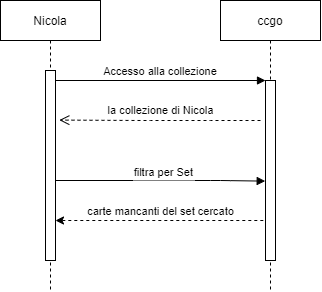
\includegraphics[height=8cm]{files/flowchart_nicola.png}
    \caption{Diagramma d'interazione per l'utente collezionista}
    \label{fig:flowchart_nicola}
\end{figure}

Iniziamo quindi con la prima query, dove Nicola vuole accedere alla pagina della sua collezione. Le informazioni che richiede sono quindi, per ogni set il numero di carte totali che lo compongono e, tra quelle, quante siano anche da lui possedute.

\begin{figure}[H]
    \centering
    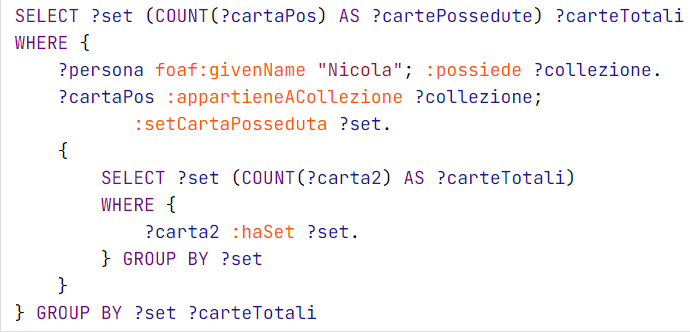
\includegraphics[width=13cm]{files/query1_nicola.png}
    \caption{Query di visualizzazione dei set di Nicola}
    \label{fig:query1_nicola}
\end{figure}

\begin{figure}[H]
    \centering
    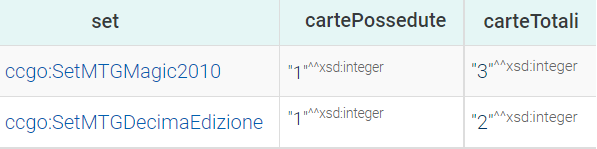
\includegraphics[]{files/res1_nicola.png}
    \caption{Lista dei Set nella collezione di Nicola}
    \label{fig:res1_nicola}
\end{figure}

Come già accennato precedentemente, i nomi dei set molto probabilmente sono univoci, proprio a causa del fatto che spesso essi sono legati all'universo narrativo del CCG di riferimento. In particolar modo questo può essere ancora più probabile se si pensa che difficilmente un utente possiederà carte da tutti i CCG esistenti, ma solo da un sottoinsieme molto ristretto composto da pochi membri. Pertanto non è necessario specificare il gioco di riferimento dei set. Nel caso dovesse invece rendersi necessario, sarebbe comunque facile da inserire modificando la query in Figura \ref{fig:query1_nicola}.

In ogni caso, a questo punto Nicola selezionerà un set, supponiamo il set "Magic 2010", per vedere quali siano esattamente le carte che gli mancano. Di seguito abbiamo la query con i relativi risultati.


\begin{figure}[H]
    \centering
    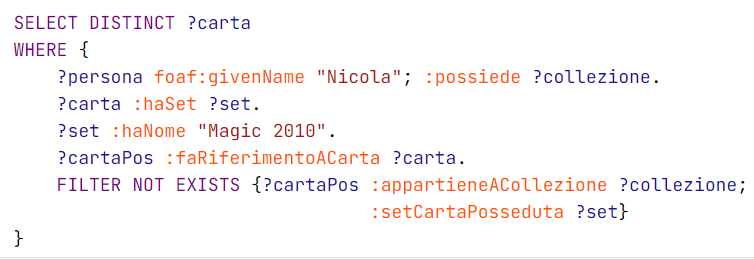
\includegraphics[width=14cm]{files/query2_nicola.png}
    \caption{Query di selezione delle carte mancanti del set "Magic 2010" di Nicola}
    \label{fig:query2_nicola}
\end{figure}

\begin{figure}[H]
    \centering
    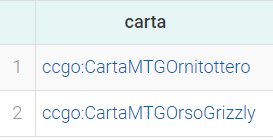
\includegraphics[]{files/res2_nicola.png}
    \caption{Lista delle carte mancanti del set "Magic 2010" di Nicola}
    \label{fig:res2_nicola}
\end{figure}

A questo punto Nicola ora sa quali carte gli manchino e può facilmente acquistarle dal suo negozio di fiducia, per completare la collezione.

\newpage
\section{Regole SWRL}
In questa sezione analizzeremo alcune regole SWRL che permettono di ampliare l'utilizzo dell'ontologia in vari modi. In particolare avremo tre categorie di regole:
\begin{enumerate}
    \item regole che asseriscono nuove proprietà \label{enum:nuove_prop}
    \item regole che impongono vincoli sulla legalità dei mazzi nei formati \label{enum:vincoli_legalita}
    \item regole che impediscono che oggetti appartenenti a giochi diversi si mischino tra loro \label{enum:giochi_diversi}
\end{enumerate}
Le sezioni seguenti sono chiamate con i nomi delle regole nell'ontologia. I dettagli saranno dati nell'analisi di ognuna di esse.
\'E tuttavia doveroso fare alcune importanti note introduttive:  l'appartenenza degli oggetti rappresentati dalle variabili alle classi corrette è garantita da domain e range delle proprietà utilizzate in ciascuna delle regole; tutte le proprietà richiamate nelle regole, con l'eccezione degli operatori built-in, di \lstinline [language=SPARQL]{sameAs} e di \lstinline [language=SPARQL]{differentFrom}, sono definite in ccgo; la disposizione di un letterale per riga è una scelta puramente stilistica per facilitare la lettura e la comprensione delle regole stesse; i nomi delle variabili è composto dalla lettera iniziale della classe a cui appartengono, eventualmente accompagnata da un pedice.


\subsection{SetCartaStessoGioco}
La prima regola che analizziamo appartiene alla categoria \ref{enum:giochi_diversi}, e impone che a una carta $c$ di un gioco $g_1$ non possa essere assegnato un set $s$ di un altro gioco $g_2$ diverso da $g_1$. Poiché in SWRL non è possibile esprimere la negazione, questa regola è stata implementata nel seguente modo.

\begin{lstlisting}[language=SPARQL]
faRiferimentoAGioco(?c, ?g1) ^ 
faRiferimentoAGioco(?s, ?g2) ^ 
haSet(?c, ?s) 
    -> 
sameAs(?g1, ?g2)
\end{lstlisting}

\subsection{CartaRistampata}
Questa regola appartiene alla categoria \ref{enum:nuove_prop} e permette di evidenziare le carte che sono state ristampate in più set, asserendo per ciascuna di esse una data property booleana.
\begin{lstlisting}[language=SPARQL]
haSet(?c, ?s1) ^ 
haSet(?c, ?s2) ^ 
differentFrom(?s1, ?s2) 
    -> 
stampataPiuVolte(?c, true)
\end{lstlisting}


\subsection{MazzoIllegale}
Questa regola appartiene alla categoria \ref{enum:vincoli_legalita} e impedisce che un mazzo sia illegale nel formato per cui è pensato. La proprietà \lstinline [language=SPARQL]{mazzoPensatoPer} permette all'utente Giocatore di specificare il formato in cui intende giocare un mazzo. Risulta quindi fondamentale che il sistema sia in grado di notificare l'utente del fatto che sta inserendo nel proprio mazzo una carta illegale nel formato per cui è pensato il mazzo stesso. In questo modo egli potrà risolvere questa incongruenza o cambiando il formato, oppure cambiando le carte illegali.

\begin{lstlisting}[language=SPARQL]
mazzoPensatoPer(?m, ?f1) ^ 
mazzoNonLegaleIn(?m, ?f2) 
    -> 
differentFrom(?f1, ?f2)
\end{lstlisting}

\subsection{MazzoDiUnSoloGioco}
Questa regola appartiene alla categoria \ref{enum:giochi_diversi} e impone che se un mazzo $m$ fa riferimento a un gioco $g_1$, allora le carte che compongono $m$ devono necessariamente appartenere tutte allo stesso gioco $g_1$.
\begin{lstlisting}[language=SPARQL]
appartieneAMazzo(?m, ?cp) ^ 
faRiferimentoACarta(?cp, ?c) ^ 
faRiferimentoAGioco(?m, ?g1) ^ 
faRiferimentoAGioco(?c, ?g2) 
    -> 
sameAs(?g1, ?g2)
\end{lstlisting}

\subsection{AssegnaGiocoAMazzo}
Questa regola appartiene alla categoria \ref{enum:nuove_prop} e permette di assegnare un gioco a un mazzo sulla base delle carte che lo compongono. In particolare, se una carta $c$ è in un mazzo $m$ e $c$ fa riferimento a un gioco $g$, allora anche $m$ deve necessariamente fare riferimento allo stesso gioco $g$.

\begin{lstlisting}[language=SPARQL]
appartieneAMazzo(?m, ?cp) ^ 
faRiferimentoACarta(?cp, ?c) ^ 
faRiferimentoAGioco(?c, ?g) 
    -> 
faRiferimentoAGioco(?m, ?g)
\end{lstlisting}

Questa regola unita alla precedente garantisce che in uno stesso mazzo non possano trovarsi carte che appartengono a giochi diversi. La regola MazzoDiUnSoloGioco da sola non è sufficiente per garantire tale condizione, infatti se un mazzo non avesse una proprietà \lstinline [language=SPARQL]{faRiferimentoAGioco}, potrebbe contenere carte da un qualsiasi numero di giochi diversi. Ciò è però impossibile a causa della regola AssegnaGiocoAMazzo che impone che un mazzo faccia riferimento al gioco di ogni carta che lo compone. 

\subsection{QuattroCopiePerMazzoModern}
Questa regola appartiene alla categoria \ref{enum:vincoli_legalita} e anche alla categoria \ref{enum:nuove_prop} e impone che un mazzo non sia legale nel formato Modern di Magic The Gathering se contiene più di 4 copie di una carta il cui tipo è diverso da "Terra Base".

\begin{lstlisting}[language=SPARQL]
appartieneAMazzo(?cp, ?m) ^ 
quantitaCarta(?cp, ?q) ^
swrlb:greaterThan(?q, 4) ^
faRiferimentoACarta(?cp, ?c) ^ 
tipoCarta(?c, ?t) ^ 
swrlb:notEqual(?t, "Terra Base") ^
Formato(?f) ^ 
haNome(?f, "Modern") ^
faRiferimentoAGioco(?f, ?g) ^
nomeGioco(?g, "Magic: The Gathering")
    -> 
mazzoNonLegaleIn(?m, ?f)
\end{lstlisting}
In maniera simile al funzionamento di questa regola sarebbe possibile esprimere altri vincoli sulla costruzione dei mazzi specifici dei vari formati. Per esempio, questa stessa regola si potrebbe ricopia cambiando solamente il massimo numero di copie permesse da 4 a 1 e il nome del formato da "Modern" a "Commander".

\end{document}